%---------change this every homework
\def\yourid{mst3k}  % substitute your userED
\def\collabs{collaborators} % substitute your collaborators
\def\sources{sources} % substitute your sources
% -----------------------------------------------------
\def\duedate{February 5, 2025 at 11:59p}
\def\pnumber{2}
%-------------------------------------

\documentclass[10pt]{article}
\usepackage{dsa2}
\usepackage{float}

\begin{document}
\thispagestyle{empty}
\handout

%----Begin your modifications here

%%%%%%%%%%%%%%%%%%%%%%%%%%%%%%%%%%%%%%%%%%%%%%%%%%%%%%%%

\begin{figure}[h]
    \centering
    \begin{tikzpicture}
        % Define nodes
        \node (A) at (0,2) {A};
        \node (B) at (2,3) {B};
        \node (C) at (4,2) {C};
        \node (D) at (2,0) {D};
        \node (E) at (6,3) {E};
        \node (F) at (8,5) {F};
        \node (G) at (6,0) {G};
        \node (H) at (4,-1) {H};

        % Draw directed edges
        \draw[->] (A) -- (B);
        \draw[->] (C) -- (B);
        \draw[->] (C) -- (D);
        \draw[->] (D) -- (A);
        \draw[->] (A) -- (C);
        \draw[->] (C) -- (E);
        \draw[->] (E) -- (F);
        \draw[->] (F) -- (G);
        \draw[->] (G) -- (H);
        \draw[->] (H) -- (D);
        \draw[->] (B) -- (F);
        \draw[->] (E) -- (G);
    \end{tikzpicture}
    \caption{Graph used for Problems 1 and 2}
    \label{fig:graph_1_2}
\end{figure}



%%%%%%%%%%%%%%%%%%%%%%%%%%%%%%%%%%%%%%%%%%%%%%%%%%%%%%%%
\begin{problem} Using Depth First Search \end{problem}

Apply depth first search starting at Node $A$ on the graph shown in Figure~\ref{fig:graph_1_2}. Use Table~\ref{tab:dfs_times} to record the seen and done timestamps (starting with 0). Note: When multiple nodes could be chosen at a given step, pick the one that comes first alphabetically (i.e. If either node F or node H could follow node C, choose node F because F is alphabetically before H.

\begin{table}[H]
    \centering
    \begin{tabular}{c|c|c}
        \toprule
        \textbf{Node} & \textbf{Seen (Discovery Time)} & \textbf{Done (Finish Time)} \\
        \midrule
        A & ?  & ? \\ %%% Student, replace these question marks
        B & ?  & ? \\
        C & ?  & ? \\
        D & ?  & ? \\
        E & ?  & ? \\
        F & ?  & ? \\
        G & ?  & ? \\
        H & ?  & ? \\
        \bottomrule
    \end{tabular}
    \caption{DFS Seen and Done Timestamps}
    \label{tab:dfs_times}
\end{table}

\newpage
%%%%%%%%%%%%%%%%%%%%%%%%%%%%%%%%%%%%%%%%%%%%%%%%%%%%%%%%
\begin{problem} Classifying Edges \end{problem}

Refer to the graph shown in Figure~\ref{fig:graph_1_2}. Use the seen and done times that you calculated above to classify the edges. For each edge choose between: Tree Edge, Back Edge, Forward Edge, Cross Edge. Use Table~\ref{tab:dfs_edges} to record your answers.

\vspace{0.3in}

\begin{table}[h]
    \centering
    \begin{tabular}{c|c}
        \toprule
        \textbf{Edge} & \textbf{Edge Type} \\
        \midrule
        (A → B) & ? Edge \\ %%% Student, replace the question marks with one of:
        (C → B) & ? Edge \\ %%%    Tree, Back, Forward, Cross
        (C → D) & ? Edge \\
        (D → A) & ? Edge \\
        (A → C) & ? Edge \\
        (C → E) & ? Edge \\
        (E → F) & ? Edge \\
        (F → G) & ? Edge \\
        (G → H) & ? Edge \\
        (H → D) & ? Edge \\
        (B → F) & ? Edge \\
        (E → G) & ? Edge \\

        \bottomrule
    \end{tabular}
    \caption{DFS Edge Types}
    \label{tab:dfs_edges}
\end{table}

\newpage
%%%%%%%%%%%%%%%%%%%%%%%%%%%%%%%%%%%%%%%%%%%%%%%%%%%%%%%%
\begin{problem} Using Dijkstra's Algorith \end{problem}

Given the following graph:

\begin{center}
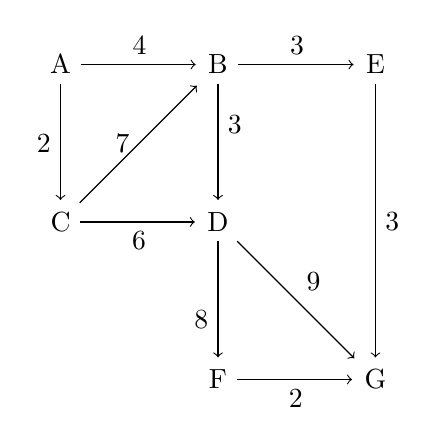
\begin{tikzpicture}[shorten >=1pt, node distance=2cm, auto]

    % Nodes
    \node (A) {A};
    \node (B) [right of=A] {B};
    \node (C) [below of=A] {C};
    \node (D) [right of=C] {D};
    \node (E) [right of=B] {E};
    \node (F) [below of=D] {F};
    \node (G) [right of=F] {G};

    % Edges with weights
    \draw[->] (A) -- (B) node[midway, above] {4};
    \draw[->] (A) -- (C) node[midway, left] {2};
    \draw[->] (B) -- (E) node[midway, above] {3};
    \draw[->] (B) -- (D) node[midway, above right] {3};
    \draw[->] (C) -- (D) node[midway, below] {6};
    \draw[->] (C) -- (B) node[midway, left] {7};
    \draw[->] (D) -- (F) node[midway, below left] {8};
    \draw[->] (D) -- (G) node[midway, above right] {9};
    \draw[->] (E) -- (G) node[midway, right] {3};
    \draw[->] (F) -- (G) node[midway, below] {2};
\end{tikzpicture}
\end{center}
\vspace{0.2in}
Apply Dijkstra's Algorithm starting at node A. Each time a decreaseKey call is made, record that in Table~\ref{tab:decreaseKey} below. Record the vertex and the value assigned. For some vertices, decreaseKey will only be called once; others might have more than one call. If decreaseKey is called more than once for a given node, there should be multiple entries in the table. There are 15 rows provided in the table, but you may not need them all, just leave the extra rows at the end of the table as they are if not needed. Note: When multiple nodes could be chosen at a given step, pick the one that comes first alphabetically (i.e. If either node F or node H could be chosen next because they have equally minimum values in the priority queue, choose node F because F is alphabetically before H).

\begin{table}[h]
    \centering
    \begin{tabular}{|c|c|c|}
        \hline
        \textbf{decreaseKey is called} & \textbf{Vertex} & \textbf{Value} \\
        \hline
        1 & A & 0 \\
        2 & ? & ? \\ %%% Student, replace the question marks with your answers
        3 & ? & ? \\
        4 & ? & ? \\
        5 & ? & ? \\
        6 & ? & ? \\
        7 & ? & ? \\
        8 & ? & ? \\
        9 & ? & ? \\
        10 & ? & ? \\
        11 & ? & ? \\
        12 & ? & ? \\
        13 & ? & ? \\
        14 & ? & ? \\
        15 & ? & ? \\ %%% Student, leave unneeded rows at the end as they are
        \hline
    \end{tabular}
    \caption{DecreaseKey Calls}
    \label{tab:decreaseKey}
\end{table}


%%%%%%%%%%%%%%%%%%%%%%%%%%%%%%%%%%%%%%%%%%%%%%%%%%%%%%%%

\end{document}
